
\newpage 

\section{Numerical Results}\label{results_section}

We now present the results from various benchmark problems in fluid-driven fracture propagation.  The problems range from those in which flow is only present within the cracks to fully coupled problems involving flow in both the matrix and the evolving manifold that is the fracture geometry. With the sole exception of the toughness-dominated KGD problem,  all of the results in this section employ the spectral split of the energy, as described in Section~\ref{sec:pfm-fracture}.  

\begin{figure}[!htbp]
\centering
\begin{subfigure}{.5\textwidth}
  \centering
  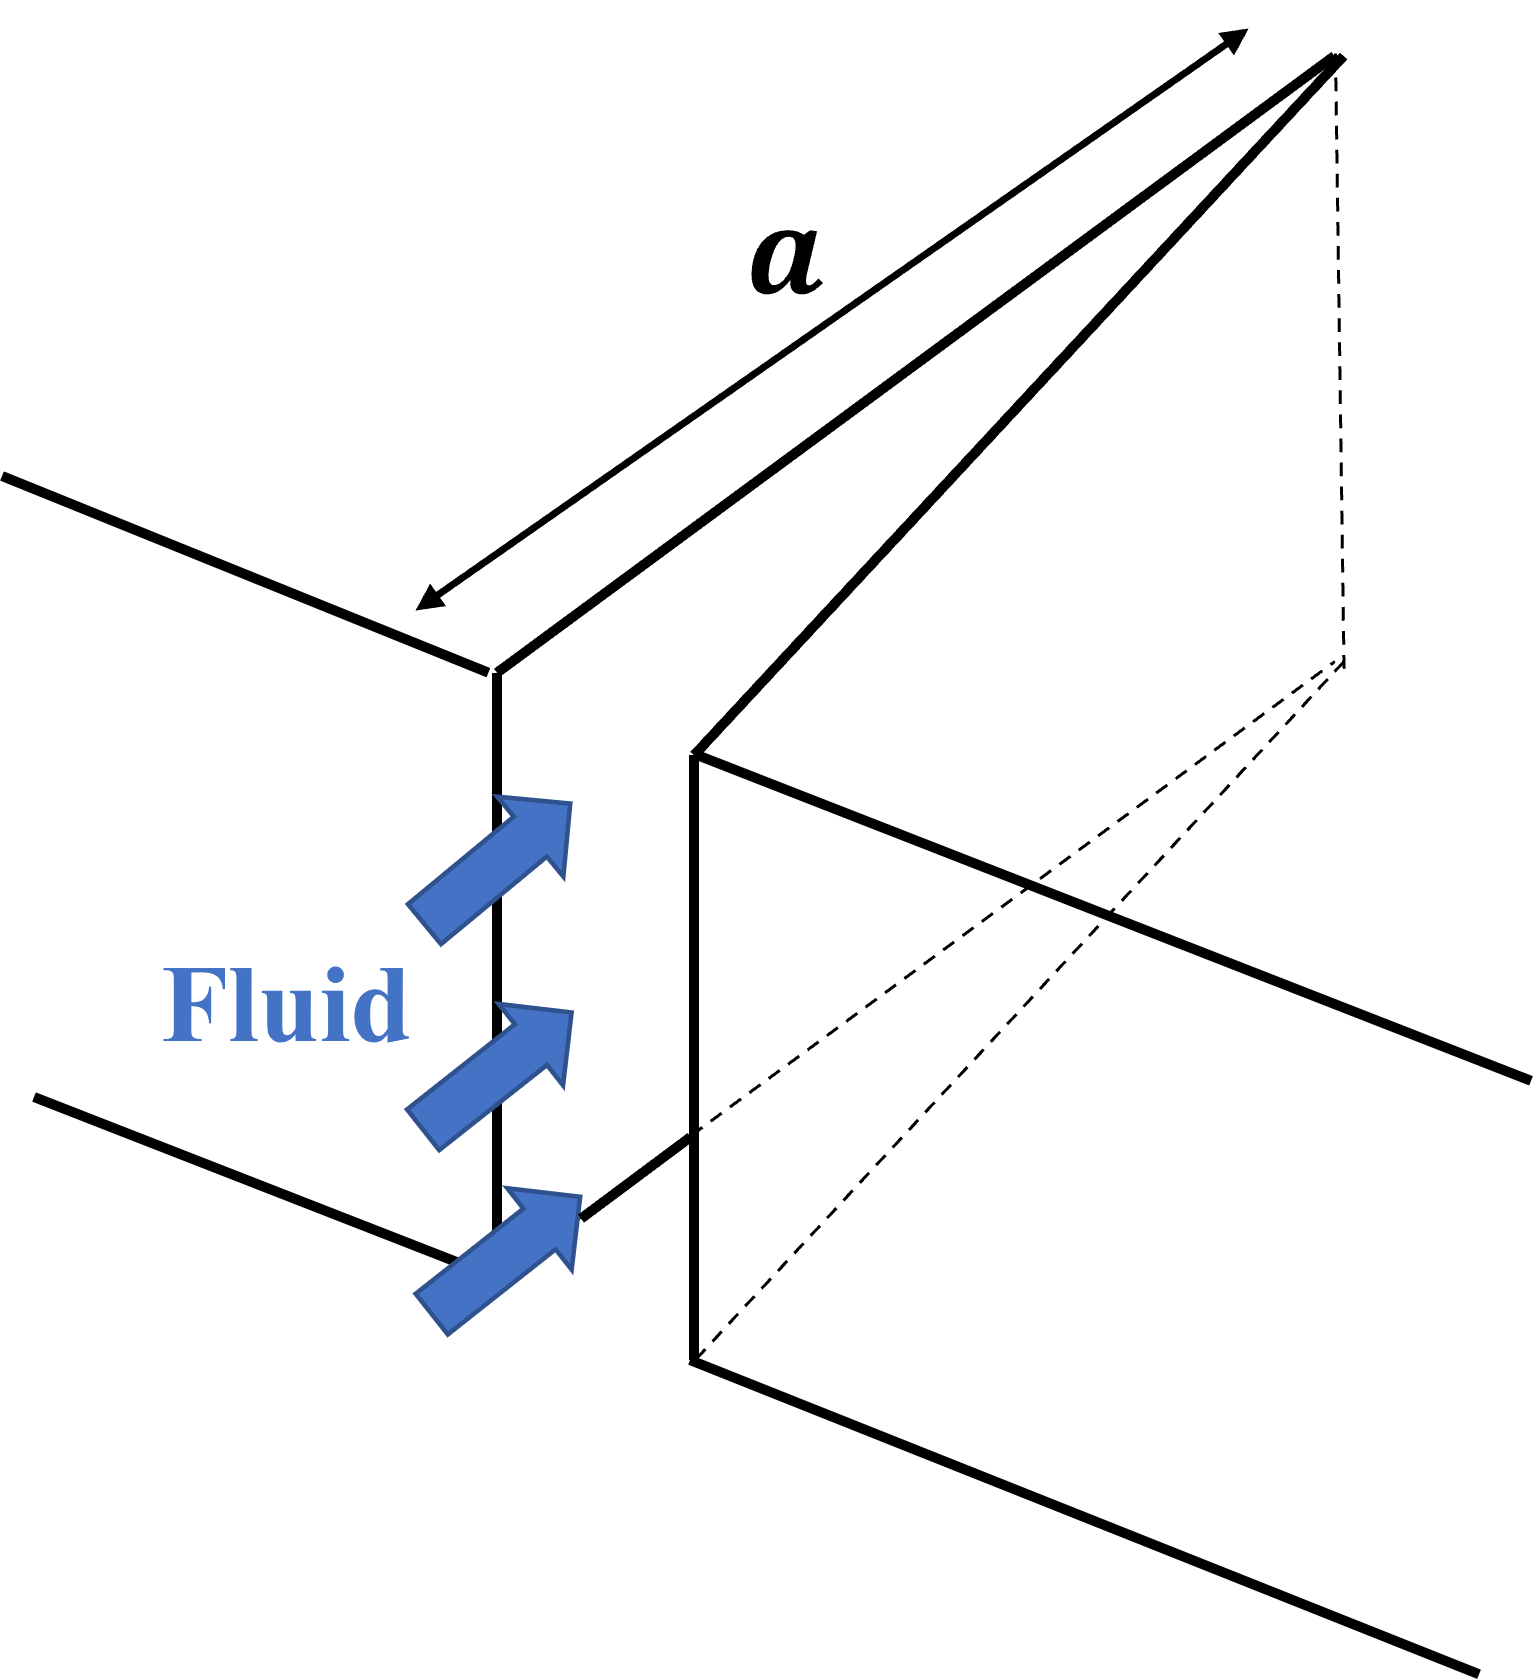
\includegraphics[width=.79\linewidth]{img/KGD_schematic_mine.png}
    \caption{}
    \label{fig:3D_schematics_kgd}
\end{subfigure}%
\begin{subfigure}{.5\textwidth}
  \centering
  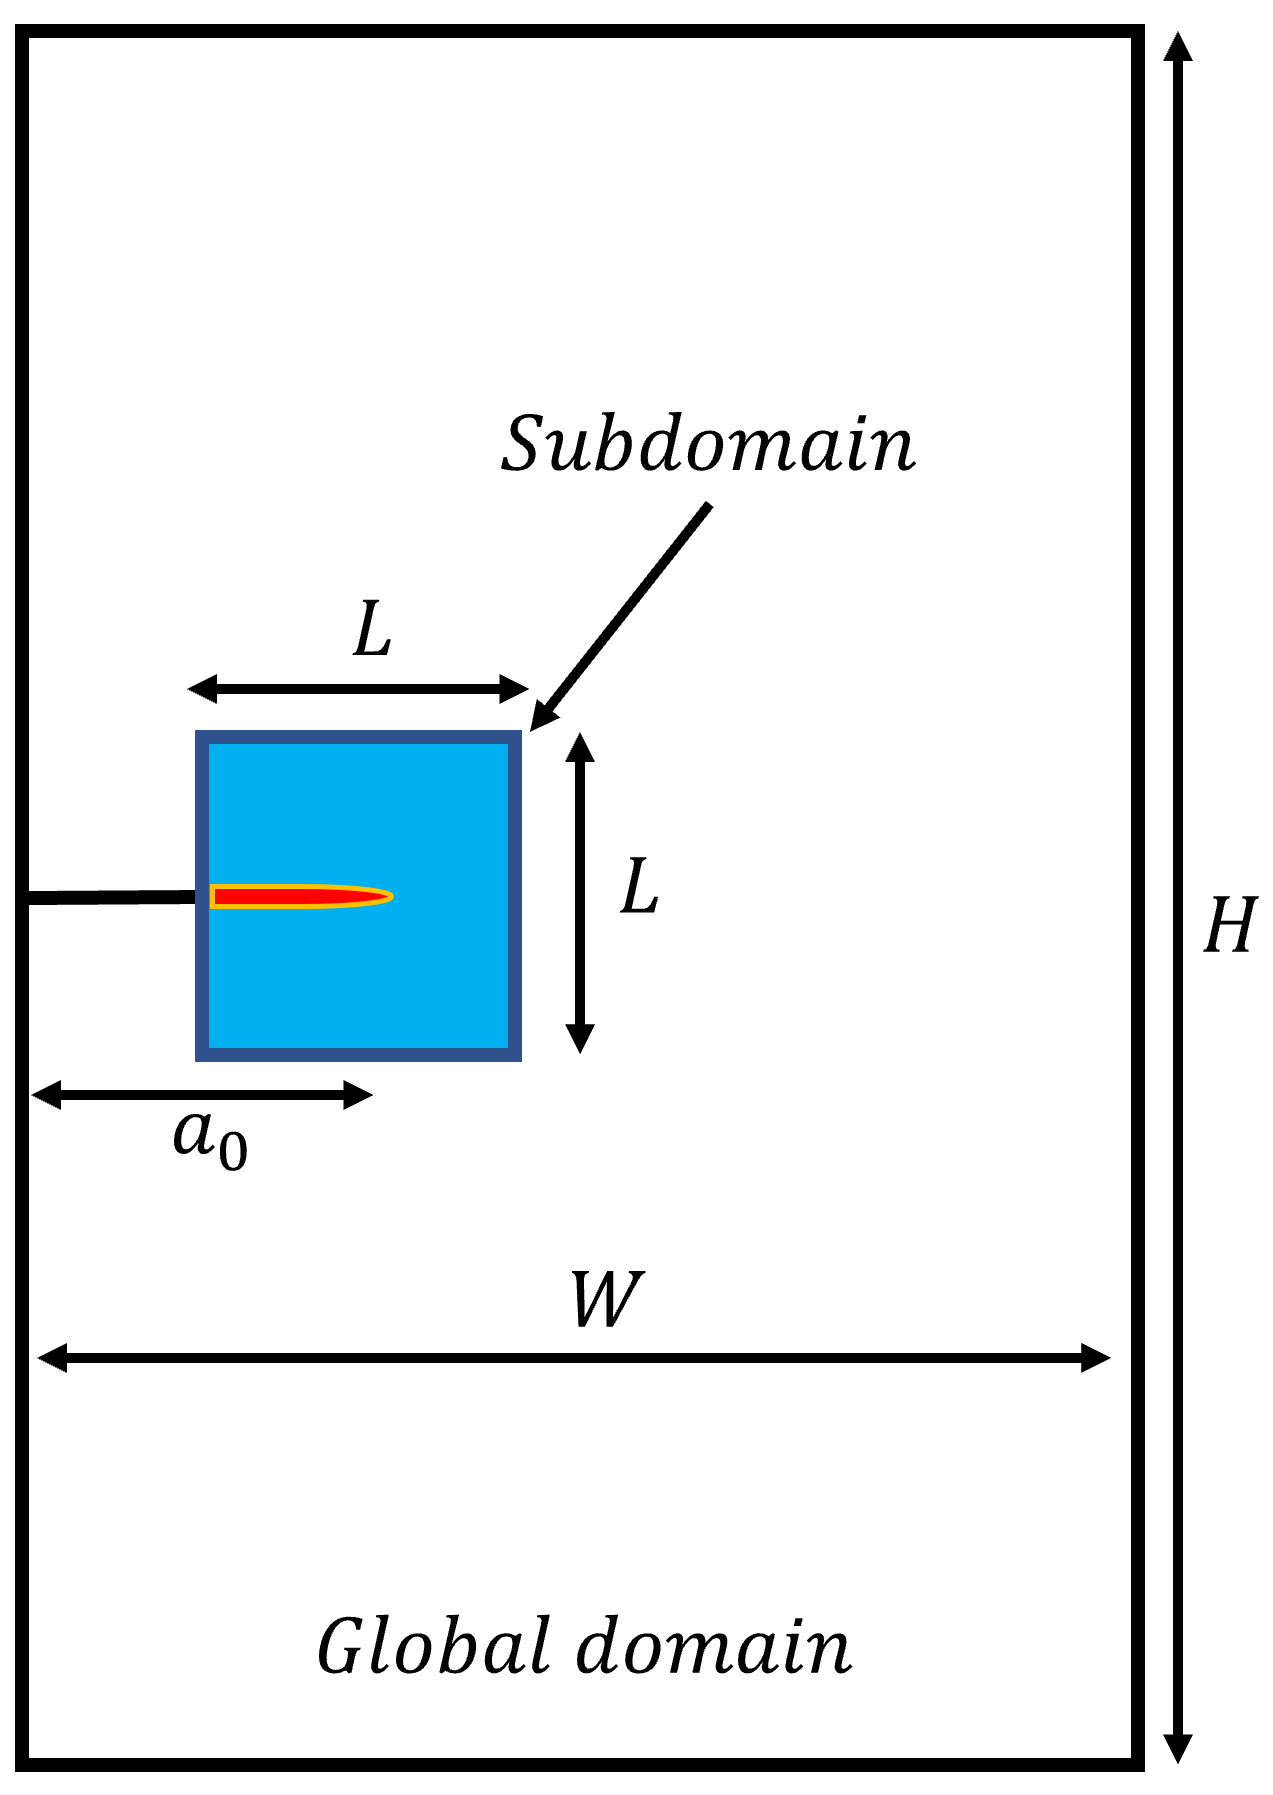
\includegraphics[width=.62\linewidth]{img/toughness_prob/KGD_schematic_2.png}
  \caption{}
  \label{fig:2D_schematics_kgd}
\end{subfigure}
\caption{(a) Schematic of the KGD problem, inspired by \cite{adachi2007computer}. (b) Computational domain for the KGD problem (not to scale).}
  \label{fig:kgd_schematics}
\end{figure}

\subsection{KGD problems} 
We begin with the well-known Khristianovic, Geertsma and De Klerk (KGD) problems of hydraulic fracture \cite{geertsma1969rapid, zheltov19553}.  The problems concern the propagation of a planar fracture in an infinite, impermeable domain, under the injection of a viscous fluid at a constant rate (Figure \ref{fig:kgd_schematics}). 

The response of the system can be characterized by the dimensionless group $\mathcal{K}$ \cite{detournay2016mechanics}:
\begin{equation}\label{KGD_group}
    \mathcal{K} = \dfrac{4G^{1/2}_{c}}{(6\pi^2E'Q\mu)^{1/4}},
\end{equation}
where $E' = E/(1-\nu^2)$. Values of $\mathcal{K} > 4$ correspond to the ``toughness dominated regime" in which crack growth is largely controlled by the fracture toughness of the media.  By contrast, when  $\mathcal{K} < 1$, the fracture toughness is relatively small and the fluid viscosity is the main factor controlling the speed of crack growth.  In the following, we explore the performance of the multi-resolution algorithm to simulate problems in both regimes.  

\subsubsection{Toughness-dominated regime}
The toughness dominated regime is characterized by the creation of new fracture surfaces accounting for almost all of the energy dissipation.  
In this scenario, the fluid can be considered to be inviscid, which leads to a constant pressure distribution over the entire crack.  The assumption of inviscid flow reduces much of the complexity, allowing for the construction of a simple analytical solution for this problem. 
Here, we consider a problem in the toughness-dominated regime resulting from the material parameters and settings given in Table \ref{parameters_tKGD}.  Using these values in \eqref{KGD_group}, we obtain $\mathcal{K} = 6.54$. 

\begin{table}[ht]
\centering
\caption{Material properties and problem parameters for the toughness-dominated KGD problem}
\begin{tabular}[t]{lcc}
\hline
&Value &Unit \\
\hline
Young's modulus ($E$)&16.0&GPa\\
Poisson's ratio ($\nu$)&0.18&--\\
Fluid viscosity ($\mu$)&1.0$\times10^{-12}$&$\text{GPa . s}$\\
Energy release rate ($G_c$)&1.85$\times10^{3}$&$\text{N/m}$\\
Injection rate ($Q$)&1.0$\times10^{-3}$&$\text{m}^2/\text{s}$\\
Initial crack size ($a_0$) &4&$\text{m}$\\
\hline
\end{tabular}
\label{parameters_tKGD}
\end{table}%

The analytical solution for this problem can be separated into two stages as a function of time. 
In the first stage, the pressure builds linearly with time and the crack does not propagate, as the pressure is below the critical threshold $p_{cr} =(G_cE'/\pi a_0)^{1/2}$.  The pressure then reaches the critical value at $t=t_{cr}$, after which the crack begins to propagate. In the second stage the propagation is stable, since the amount of fluid injected is finite and crack propagation leads to a pressure drop as the total space available for the fluid to occupy increases.

The solution for the crack length and pressure in the crack can be written as

\begin{equation}\label{length_solution_tkgd}
    a(t) =     \begin{cases}
      a_0, &  t \le t_{cr},  \\
      \left(\dfrac{E'(Qt)^2}{\pi G_c}\right)^{1/3}, &  t \ge t_{cr}, 
    \end{cases}
\end{equation}

\begin{equation}\label{pressure_solution_tkgd}
    p(t) =     \begin{cases}
      \dfrac{t}{t_{cr}}p_{cr}, &  \ t \le t_{cr},\\
      \left(\dfrac{E'G_c^2}{\pi Qt}\right)^{1/3}, &  t \ge t_{cr},
    \end{cases}
\end{equation}

\noindent where $t_{cr} =(\pi G_c a_0^3/Q^2E')^{1/2}$. A derivation of this solution can be found in Yoshioka \cite{yoshioka2020crack}.

For simulations using the multi-resolution scheme, a computational domain of size $W\times H = 30\text{ m} \times 240\text{ m}$ is used (Figure \ref{fig:2D_schematics_kgd}). According to \cite{isida1973analysis}, this domain size should be sufficiently large to yield a good approximation to an infinite plane.  We first report results using a sub-domain size of $L \times L = a_0 \times a_0$.   The sensitivity of the results to the choice of sub-domain size will be discussed later in this subsection.  

In what follows, we report results from a refinement study.  In particular, we report results for three different regularization lengths of decreasing value, beginning with $\ell = a_0/15$.  As the regularization length is decreased, we maintain a mesh size in the subdomain of $h_{local} = \ell/{4}$.  This allows the finite-element approximation to sufficiently resolve the regularized fracture band. We also note that the effective fracture toughness in the computational problem depends on $h/\ell$ \cite{yoshioka2020crack}.  In the global domain, we maintain the mesh spacing at the ratio of $h_{global} = 3h_{local}$.  For the coarsest global mesh, this translates into roughly 20 elements over the span of the initial crack geometry.  This level of resolution is consistent with those found to be sufficient for resolving pressurized cracks using the Embedded Finite Element Method, in Cusini et al.\ \cite{cusini2021simulation}.

The results obtained with the multi-resolution scheme are compared to the analytical solutions \ref{length_solution_tkgd} and \ref{pressure_solution_tkgd} in Figures \ref{fig:tkgd_length} and \ref{fig:tkgd_pressure}. We note the overall good match between the simulation results and the analytical solution, as well as the convergence of the results towards \ref{length_solution_tkgd} and \ref{pressure_solution_tkgd} when $\ell$ decreases. Although this problem is relatively simple as the matrix is assumed to be impermeable, it does test the coupling between the global and the local domains and verifies that the phase-field method, even when used only in a vicinity of the crack tip, can still provide accurate predictions of fracture propagation. Although the spectral split was not employed for this problem, we did examine the results using it.  Qualitatively they were found to be very similar, with slightly less accuracy in the calculated values of the critical pressure.   

\begin{figure}
\centering
\begin{subfigure}{.5\textwidth}
  \centering
  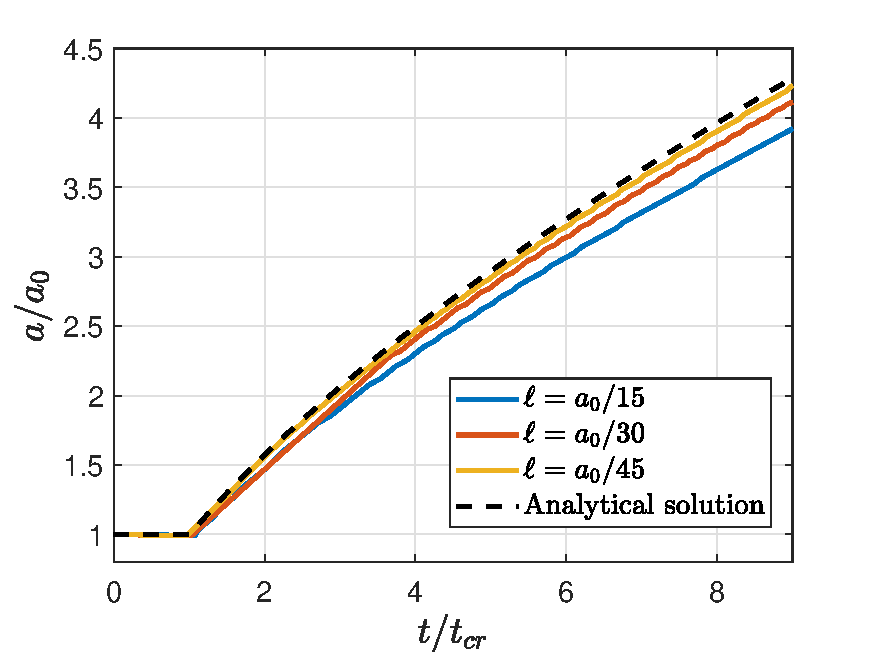
\includegraphics[width=.99\linewidth]{img/toughness_prob/length_tkgd}
  \caption{}
  \label{fig:tkgd_length}
\end{subfigure}%
\begin{subfigure}{.5\textwidth}
  \centering
  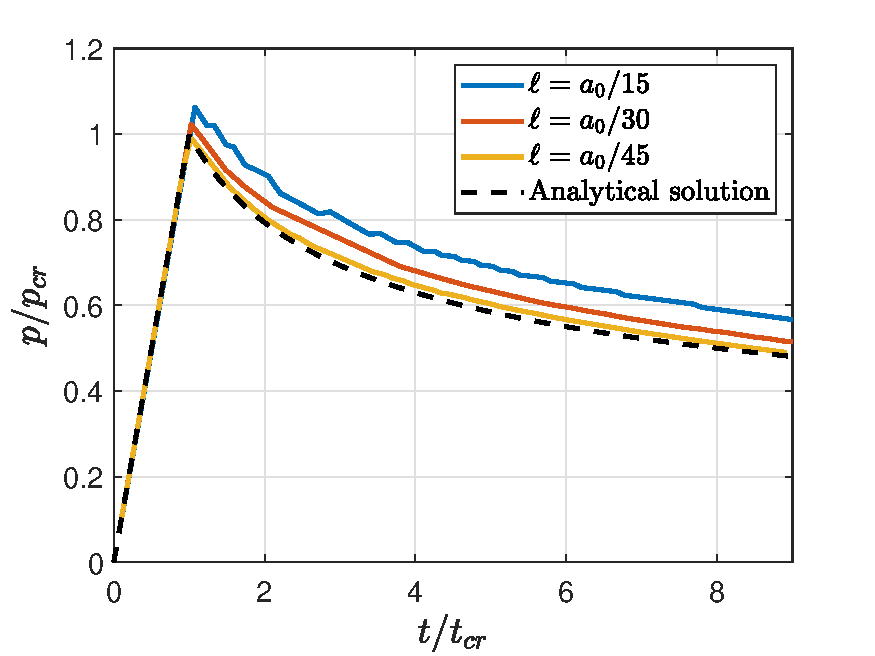
\includegraphics[width=.99\linewidth]{img/toughness_prob/pressure_tkgd}
  \caption{}
  \label{fig:tkgd_pressure}
\end{subfigure}
\caption{Comparison of numerical results and analytical solution for the toughness-dominated KGD problem: (a) crack length vs.\ time and (b) pressure vs.\ time.}
  \label{fig:tkgd_charts}
\end{figure}
\FloatBarrier

We now examine the sensitivity of the results to changes in the subdomain size.  This is accomplished by fixing the sizes of the global and local meshes as well as the regularization length, and varying only $L$ in Figure \ref{fig:2D_schematics_kgd}. In particular, we fix the regularization length to $\ell = 0.13\text{ m}$ and vary the sub-domain size between $15\ell$ and $45\ell$.  

Figures \ref{fig:adjusting_L_a} and \ref{fig:adjusting_L_p} provide the results for the pressure and crack length as a function of time, for the various choices of subdomain size. Table \ref{subdomain_size_table} shows the error in the computation of the crack length relative to the analytical solution.  The error is taken as an average over the time range, starting at the beginning of propagation.

\begin{figure}[!htbp]
\centering
\begin{subfigure}{.5\textwidth}
  \centering
  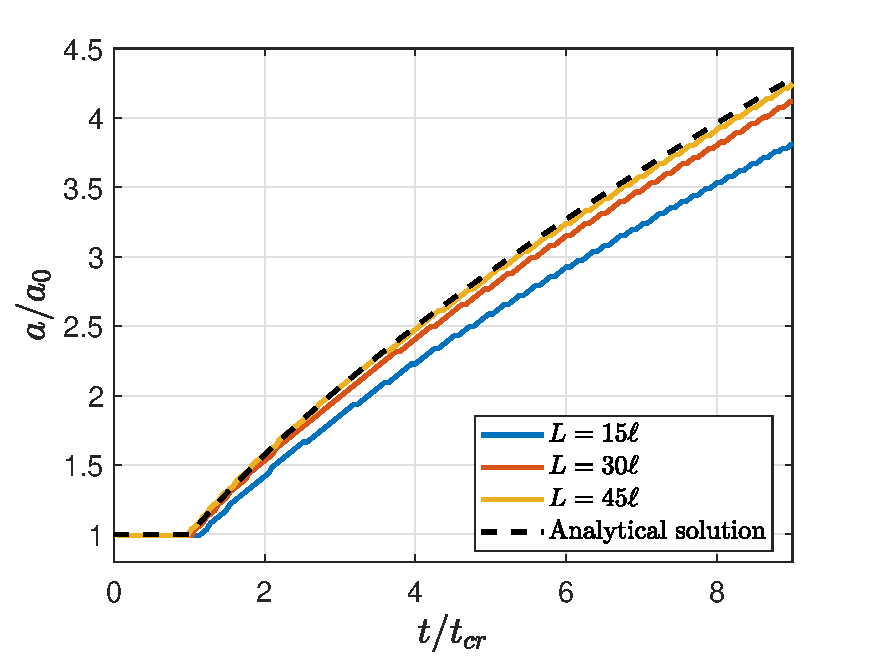
\includegraphics[width=\linewidth]{img/toughness_prob/length_L_analysis}
  \caption{}
  \label{fig:adjusting_L_a}
\end{subfigure}%
\begin{subfigure}{.5\textwidth}
  \centering
  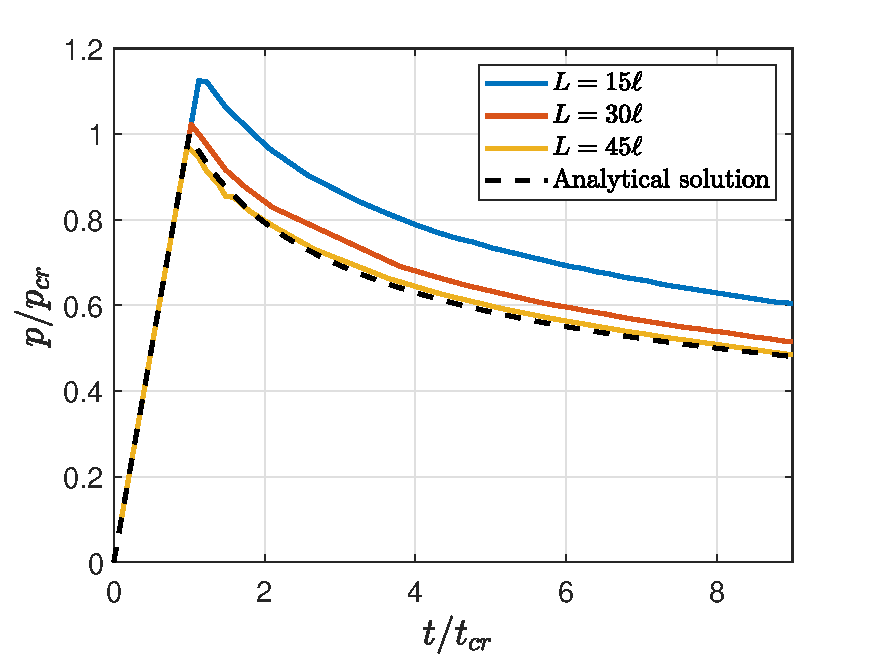
\includegraphics[width=\linewidth]{img/toughness_prob/pressure_L_analysis}
  \caption{}
  \label{fig:adjusting_L_p}
\end{subfigure}
  \caption{Study of the effects of subdomain size on the results of the toughness-dominated KGD problem:  (a) influence on predicted crack length and (b) predicted pressure. }
  \label{fig:adjusting_L}
\end{figure}
\FloatBarrier

\begin{table}[ht]
\centering
\caption{Effect of subdomain size on the relative error in the crack length. }
\begin{tabular}[t]{lcccc}
\hline
Subdomain size &Relative error   \\
\hline
$L = 15\ell$&11.5\%&\\
$L = 30\ell$&3.3\%&\\
$L = 45\ell$&1.1\%&\\

\hline
\end{tabular}
\label{subdomain_size_table}
\end{table}%

The results indicate that the error reduces as the subdomain size is increased.  In this particular study, both the global and subdomain meshes are fairly refined, and so the improvement in accuracy as $L$ increases is not likely due simply to better resolution in the local subdomain.  Rather, it may be due to the fact that the two problems are coupled through the global displacements applied to the subdomain boundary.  As the subdomain size is increased, the boundary of the subdomain moves farther from the crack tip singularity, and one would expect a better correspondence between the displacement fields obtained from the global problem and those obtained using a phase-field approximation over the entire domain.  Furthermore, as the global displacements are held fixed until the regularized crack advances sufficiently far, there is some sensitivity of the proximity of the regularized crack tip to the subdomain boundary.  

In more general cases, one would expect the subdomain mesh to be at quite a bit higher resolution than the global mesh. Since the phase-field problem also requires several iterations in the alternate minimization scheme, problems are expected to become much more computationally expensive as $L$ is increased. As a result, a trade-off between accuracy and computational cost is to be expected.  In general, one should select  a subdomain size that strikes a balance between being large enough to capture the crack evolution and small enough to render the overall calculation efficient. 

\subsubsection{Viscosity dominated KGD problem}

We now consider a case in which the choice of parameters gives rise to conditions wherein the energy dissipation is dominated by viscous dissipation.  In particular, we consider the material properties and problem parameters provided in Table~\ref{parameters_vKGD}.  Consistent with \eqref{KGD_group}, these values give rise to $\mathcal{K} = 0.57$, a result that is clearly within the viscosity-dominated regime.   

\begin{table}[ht]
\centering
\caption{Material properties and problem parameters for the viscosity-dominated KGD problem}
\begin{tabular}[t]{lcc}
\hline
&Value &Unit \\
\hline
Young's modulus ($E$)&0.17&GPa\\
Poisson's ratio ($\nu$)&0.20&--\\
Fluid viscosity ($\mu$)&1.0$\times10^{-10}$&$\text{GPa . s}$\\
Energy release rate ($G_c$)&21&$\text{N/m}$\\
Injection rate ($Q$)&1.0$\times10^{-3}$&$\text{m}^2/\text{s}$\\
Initial crack size ($a_0$) &4.0&$\text{m}$\\
\hline
\end{tabular}
\label{parameters_vKGD}
\end{table}%

In this scenario, the toughness of the medium can be neglected, and the fracture evolution is effectively dictated by the motion of the fluid front.  In this case, the pressure varies with time and space over the length of the fracture surface.   Although this problem does not include a pressure field in the matrix,  it bears emphasis that it does require the transfer of the pressure field in the fracture from the global scale to the phase-field problem in the subdomain.  As such, it serves as a test of that aspect of the multi-resolution scheme. The presence of dynamic terms in the fluid equation also implies the need for a discretization with sufficiently accurate temporal resolution, and in what follows we examine the sensitivity of the results to the choice of the time step size.  

Once again, consider a computational domain with dimensions $W\times H = 30\text{ m} \times 240\text{ m}$.  The sub-domain size is taken as $L \times L = a_0 \times a_0$, and the regularization length is taken to be $\ell = a_0/15$.  In contrast to what we observed for the toughness regime, we note that the results to the viscosity-dominated problem were found to be largely insensitive to the choice of the regularization length, provided that $\ell < a_0/10$.  This is not surprising, given that the phase-field subproblem only serves to propagate a crack that has effectively zero toughness.

In what follows, we report results using mesh spacings in the local and global domains of $h_{local} = \ell/{4}$ and $h_{global} = 3h_{local}$.  As an initial condition, the pressure field is prescribed to match the analytical solution. We report on the temporal convergence of results obtained using fixed time steps, beginning with $\text{dt}_0 = 0.5$s.  As (discrete) negative pressures arose in our simulations, the phase-field model was modified to account for a tension-compression asymmetry.  In particular, consistent with the model described in Miehe et al. \cite{miehe2010phase}, the strain energy density was split into active and inactive parts, and only the ``tensile" part was degraded with the damage.  

\begin{figure}[!htbp]
\centering
\begin{subfigure}{.5\textwidth}
  \centering
  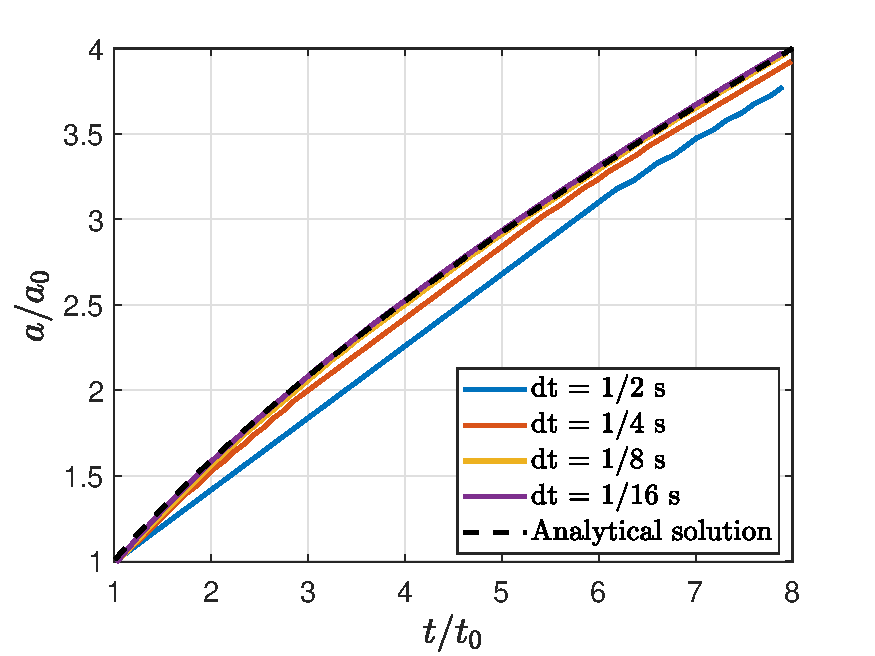
\includegraphics[width=.99\linewidth]{img/viscosity_prob/vkgd_noaeff_length_paper}
  \caption{}
  \label{fig:vkgd_length}
\end{subfigure}%
\begin{subfigure}{.5\textwidth}
  \centering
  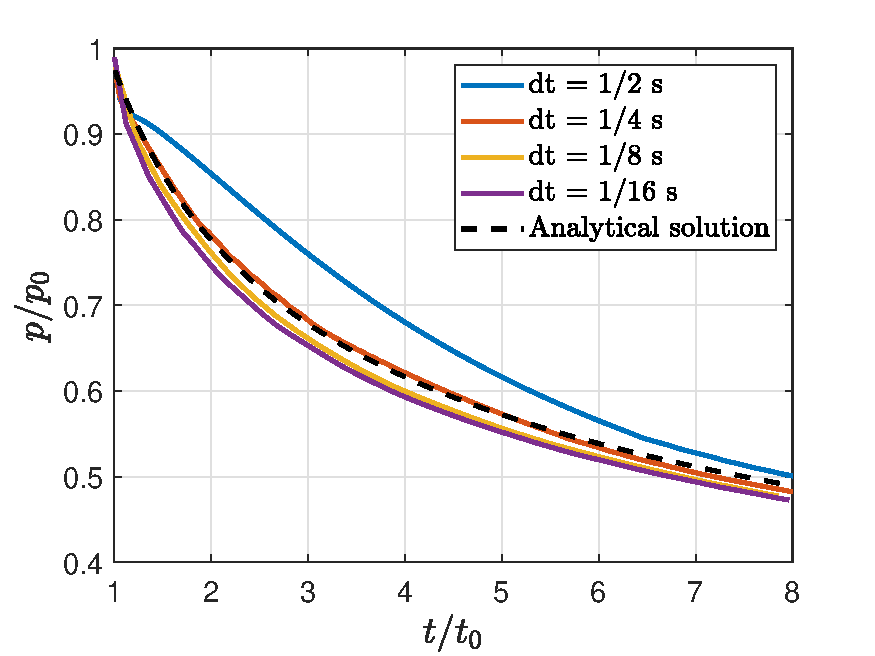
\includegraphics[width=.99\linewidth]{img/viscosity_prob/vkgd_noaeff_paper}
  \caption{}
  \label{fig:vkgd_pressure}
\end{subfigure}
\caption{Numerical results and analytical solution for the viscosity-dominated KGD problem: (a) crack length vs.\ time; and (b) inlet pressure vs.\ time. 
}
  \label{fig:vkgd_charts}
\end{figure}

Figure~\ref{fig:vkgd_charts} compares the analytical solutions for the crack length and inlet pressure to the model-based simulation results for a sequence of decreasing time steps.   The initial  time ($t_0 = 8.5 \text{ s}$), initial inlet pressure ($p_0 = 40 \text{ kPa}$) and initial crack size ($a_0 = 4\text{ m}$) were used to render the results dimensionless.   The particular values of $t_0$ and $p_0$ were chosen in order to make our initial state a snapshot of the analytical solution. Overall, the good agreement between the results indicates that the multi-resolution scheme is capable of handling a viscosity-dominated case.    

The results for the crack length show an excellent agreement with the analytical solution as the time step is decreased. The results for the inlet pressure (Figure~\ref{fig:vkgd_charts}b) appear to converge to a trajectory that is slightly offset from the analytical solution as the time step is decreased.  This relatively small discrepancy  can be explained by the presence of a minimum aperture that is assigned to the newly-initialized finite volumes in the flow solver.  As explained in \cite{settgast2017fully}, this is necessary to preserve the stability of the scheme when new crack segments are added. The recent work by Jin et al.~\cite{jin2022robust} proposes a method for removing this parameter by employing partially fractured elements. The incorporation of similar modifications in the context of the multi-resolution scheme is the subject of future work. 

\subsection{Poroelastic problem with coupled matrix-fracture flow }

\begin{figure}[!htbp]
    \centering
    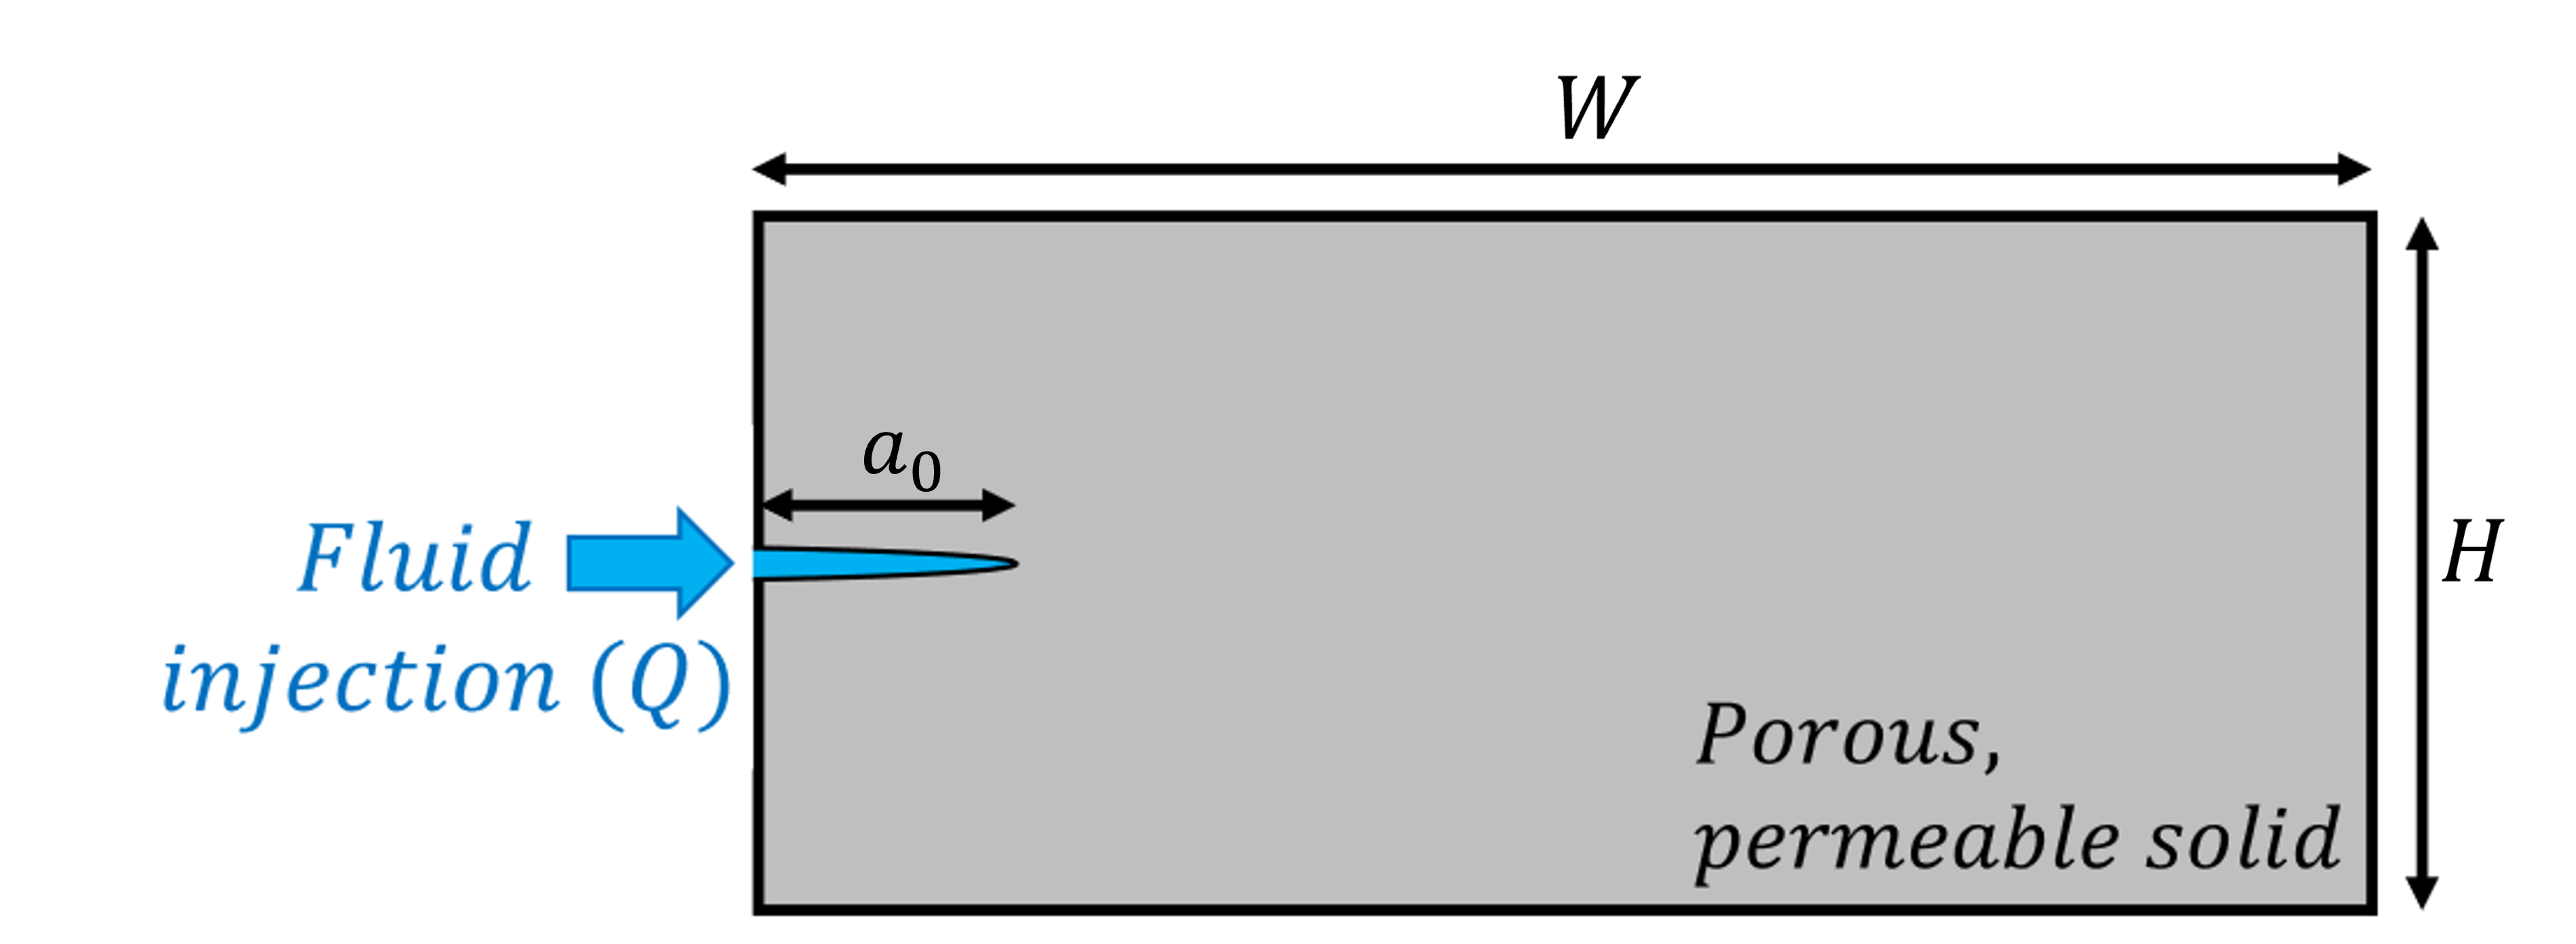
\includegraphics[width=.9\linewidth]{img/comparison_prob/miehe_prob_schematic.png}
    \caption{Geometry and notation for the coupled poroelastic-fracture problem.}
    \label{fig:geometry_miehe}
\end{figure}

We now examine a problem in which the matrix is permeable and there is a coupling between the fluid flow in the fracture, fluid flow in the matrix, and crack propagation.  A schematic of the problem is shown in Figure~\ref{fig:geometry_miehe}.   It corresponds to a rectangular domain subject to the injection of a viscous fluid at the mouth of an initial fracture.  The fluid injection rate $Q$ is assumed to be constant, and the displacement in the normal direction is fixed on all sides of the domain.  

Although this problem is relatively simple, to our knowledge an analytical solution is not available.  In what follows, we therefore compare our results to those that are obtained using an existing phase-field method for hydraulic fracture.  In particular, we compare our results to those obtained using the method described by Miehe and Mauthe \cite{miehe2015minimization, miehe2016phase}.  This is arguably one of the simpler methods available for this class of problems, combining the equations for phase-field fracture, Biot's theory of linear poroelasticity in the matrix, and lubrication theory for fluid flow within fractures.

The model assumes that a Darcy model of flow holds in the matrix, with isotropic permeability.  In the fractures, a lubrication flow model is assumed.  The transition between the two flow regimes is effected through the use of a permeability tensor that varies as a function of the crack aperture and orientation.  In particular, the permeability tensor ${\boldsymbol{\kappa}}$ is given by
\begin{equation}\label{miehe_model_basics}
    \boldsymbol{\kappa} = \boldsymbol{\kappa}_0 + d^\xi\dfrac{w^2_n}{12}\left(\textbf{I} - \textbf{n}^d \otimes \textbf{n}^d \right),
\end{equation}

\begin{equation}\label{miehe_model_aperture}
    w_n = h (\textbf{n}^d \cdot \bf{\epsilon} \cdot \textbf{n}^d),
\end{equation}

\noindent in which the normalized gradient $\textbf{n}^d = \nabla d/|\nabla d|$ approximates the normal to the crack plane.   In the above, $\boldsymbol{\kappa}_0$ is an isotropic part of the permeability that accounts for the undamaged permeability of the matrix, $w_n$ is the crack's normal aperture, and $\xi$ is a weighting exponent.  The weighting exponent concentrates the effects of the second term in \ref{miehe_model_basics} to areas where $d \approx 1$. Consistent with the work of Miehe and Mauthe \cite{miehe2015minimization, miehe2016phase}, we use $\xi= 50$.

\begin{table}[ht]
\centering
\caption{Material properties for poroelastic problem}
\begin{tabular}[t]{lcc}
\hline
&Value &Unit \\
\hline
Young's modulus ($E$)&16.0&GPa\\
Poisson's ratio ($\nu$)&0.18&--\\
Fluid viscosity ($\mu$)&1.0$\times10^{-12}$&$\text{GPa . s}$\\
Energy release rate ($G_c$)&3.67&$\text{N/m}$\\
Biot coefficient ($\alpha$)&0.79&$\text{ - }$\\
Rock permeability ($\boldsymbol{\kappa_0}$)&1.0$\times 10^{-13}$&$\text{m}^2$\\
\hline
\end{tabular}
\label{material properties miehe}
\end{table}%

\begin{table}[ht]
\centering
\caption{Problem settings}
\begin{tabular}[t]{lcc}
\hline
&Value &Unit \\
\hline
Phase-Field reg. length ($\ell$)&0.2&m\\
Subdomain size ($L$) &4.0&m\\
Domain width ($W$) &30&$\text{m}$\\
Domain height ($H$) &10&$\text{m}$\\
Initial crack size ($a_0$) &4.0&$\text{m}$\\
Injection rate ($Q$)&1.0$\times10^{-3}$&$\text{m}^2/\text{s}$\\
\hline
\end{tabular}
\label{geometry properties miehe}
\end{table}%

\medskip

The material properties used in this problem are given in Table~\ref{material properties miehe}, while the problem and model parameters are provided in Table~\ref{geometry properties miehe}.  The results reported in this section rely on the use of an eigen-decomposition of the strain energy, as described in Miehe et al. \cite{miehe2010phase}.  The subdomain size for the multi-resolution method was chosen to be proportional to the initial crack size, or $a_0 \times a_0$. The problem was discretized spatially using a uniform mesh  in the local domain with  $h_{local} = \ell/4$, while $h_{global} = 3h_{local}$ was used in the global domain. For the temporal discretization, a uniform time step of $\text{dt} = 0.125\text{ s}$ was used.  This level of spatial and temporal discretization was found to yield results that were sufficiently converged.  

An important difference between the phase-field formulation used in Miehe and Mauthe \cite{miehe2015minimization, miehe2016phase} and that employed in the current multi-resolution method concerns the use of pressure-dependent driving forces.  We draw the reader's attention to the terms involving the pressure fields $p_m$ and $p_f$ in the evolution equation \eqref{damage equation ch3} for the damage field.  In our studies of the KGD problem, we found these terms necessary to include in order to obtain sufficiently accurate simulations.  We refer to these terms as ``driving pressures" as the pressure fields contribute directly to the evolution of the damage field.  Importantly, the phase-field formulation of Miehe and Mauthe \cite{miehe2015minimization, miehe2016phase} does not include these terms in the damage evolution equation.   Accordingly, in what follows we find it useful to compare results from Miehe and Mauthe \cite{miehe2015minimization, miehe2016phase} to those obtained using our multi-resolution method with and without the driving pressures.  

\begin{figure}
\centering
\vspace{-\abovedisplayskip}
\begin{subfigure}{.5\textwidth}
  \centering
  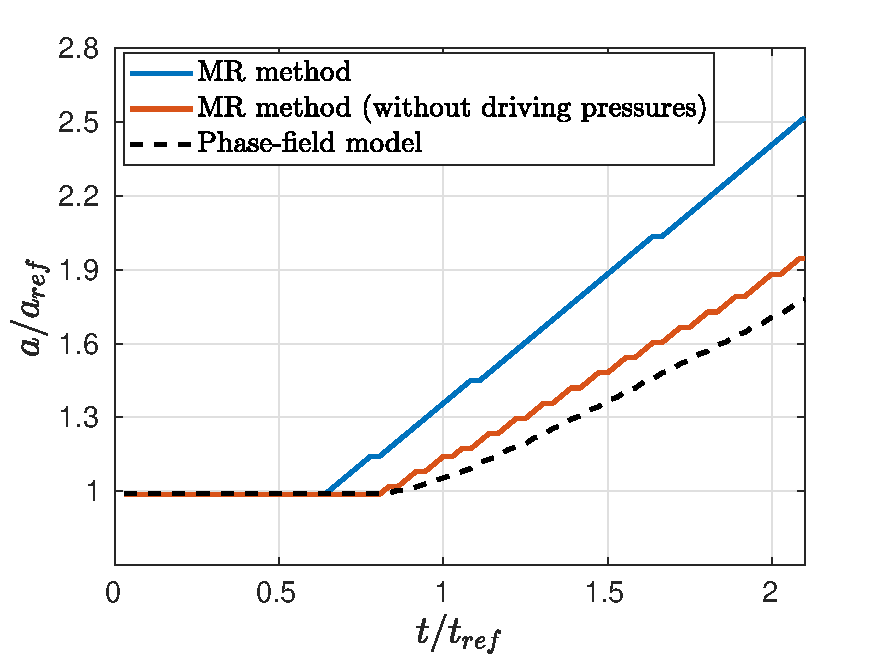
\includegraphics[width=\linewidth]{img/comparison_prob/length.pdf}
  \caption{}
  \label{fig:results_size_miehe}
\end{subfigure}%
\begin{subfigure}{.5\textwidth}
  \centering
  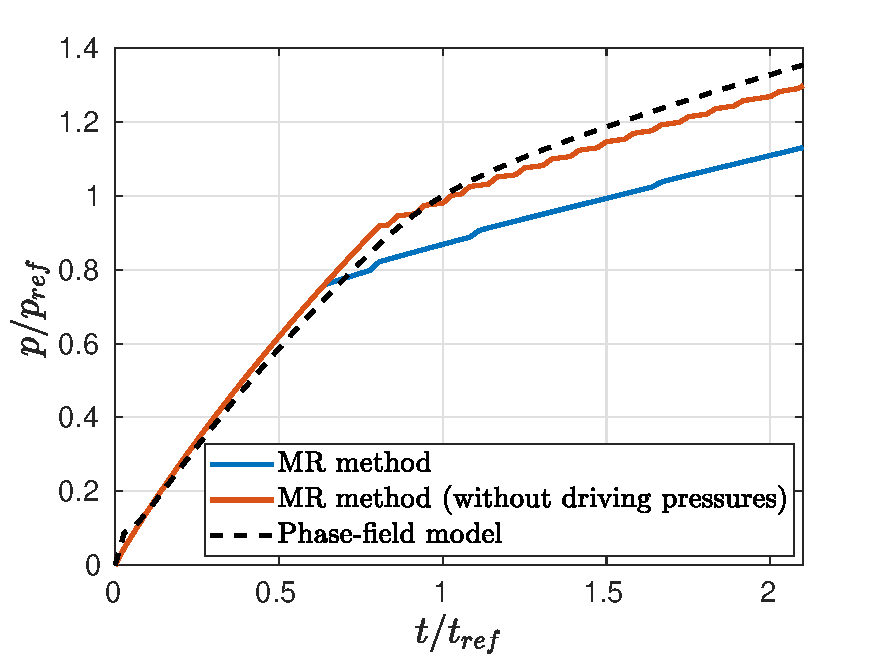
\includegraphics[width=\linewidth]{img/comparison_prob/pressures.pdf}
  \caption{}
  \label{fig:results_pressure_miehe}
\end{subfigure}
  \caption{Results from the fully coupled poroelastic-fracture problem for the multi-resolution method (with and without driving pressures) and a standard phase-field model: (a) crack size over time, (b) inlet pressure.  The time for crack propagation ($t_{ref}$) in the phase-field model and the corresponding inlet pressure ($p_{ref}$) are used as references for the dimensionless charts above.}
  \label{fig:results_charts_miehe}
\end{figure}

% \medskip
\medskip

\begin{figure}
\centering
\vspace{-\abovedisplayskip}
\begin{subfigure}{.5\textwidth}
  \centering
  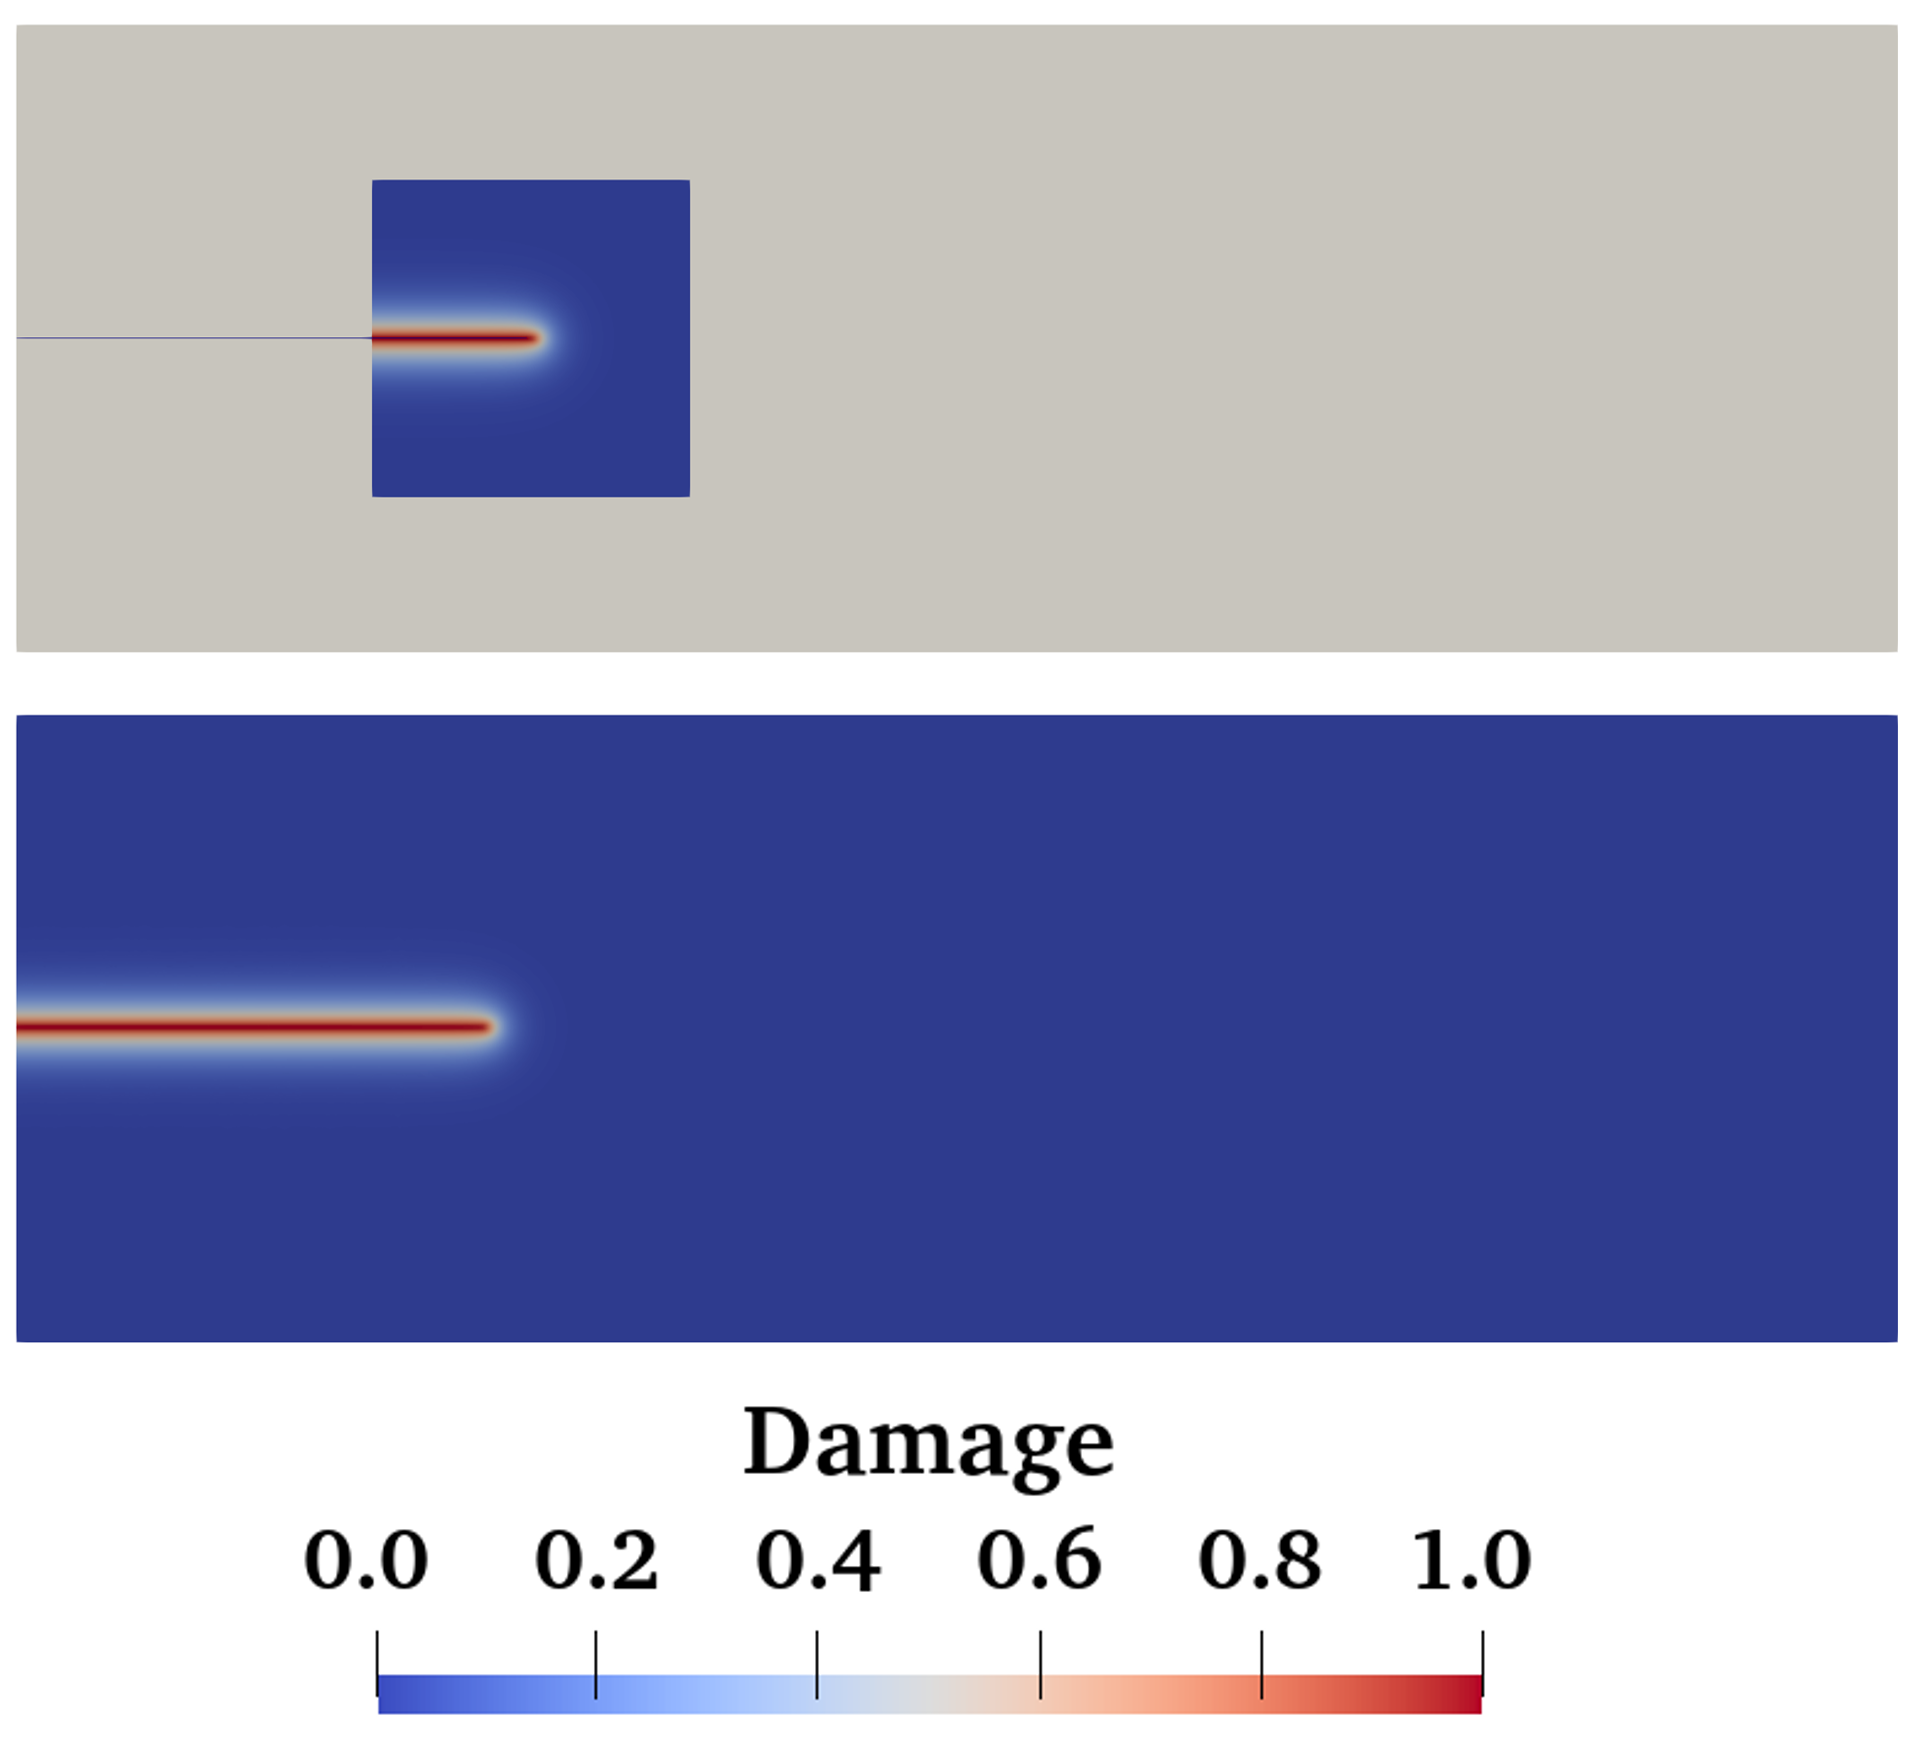
\includegraphics[width=\linewidth]{img/comparison_prob/damage_fields.png}
  \caption{}
  \label{fig:damage_snapshot_p2}
\end{subfigure}%
\begin{subfigure}{.5\textwidth}
  \centering
  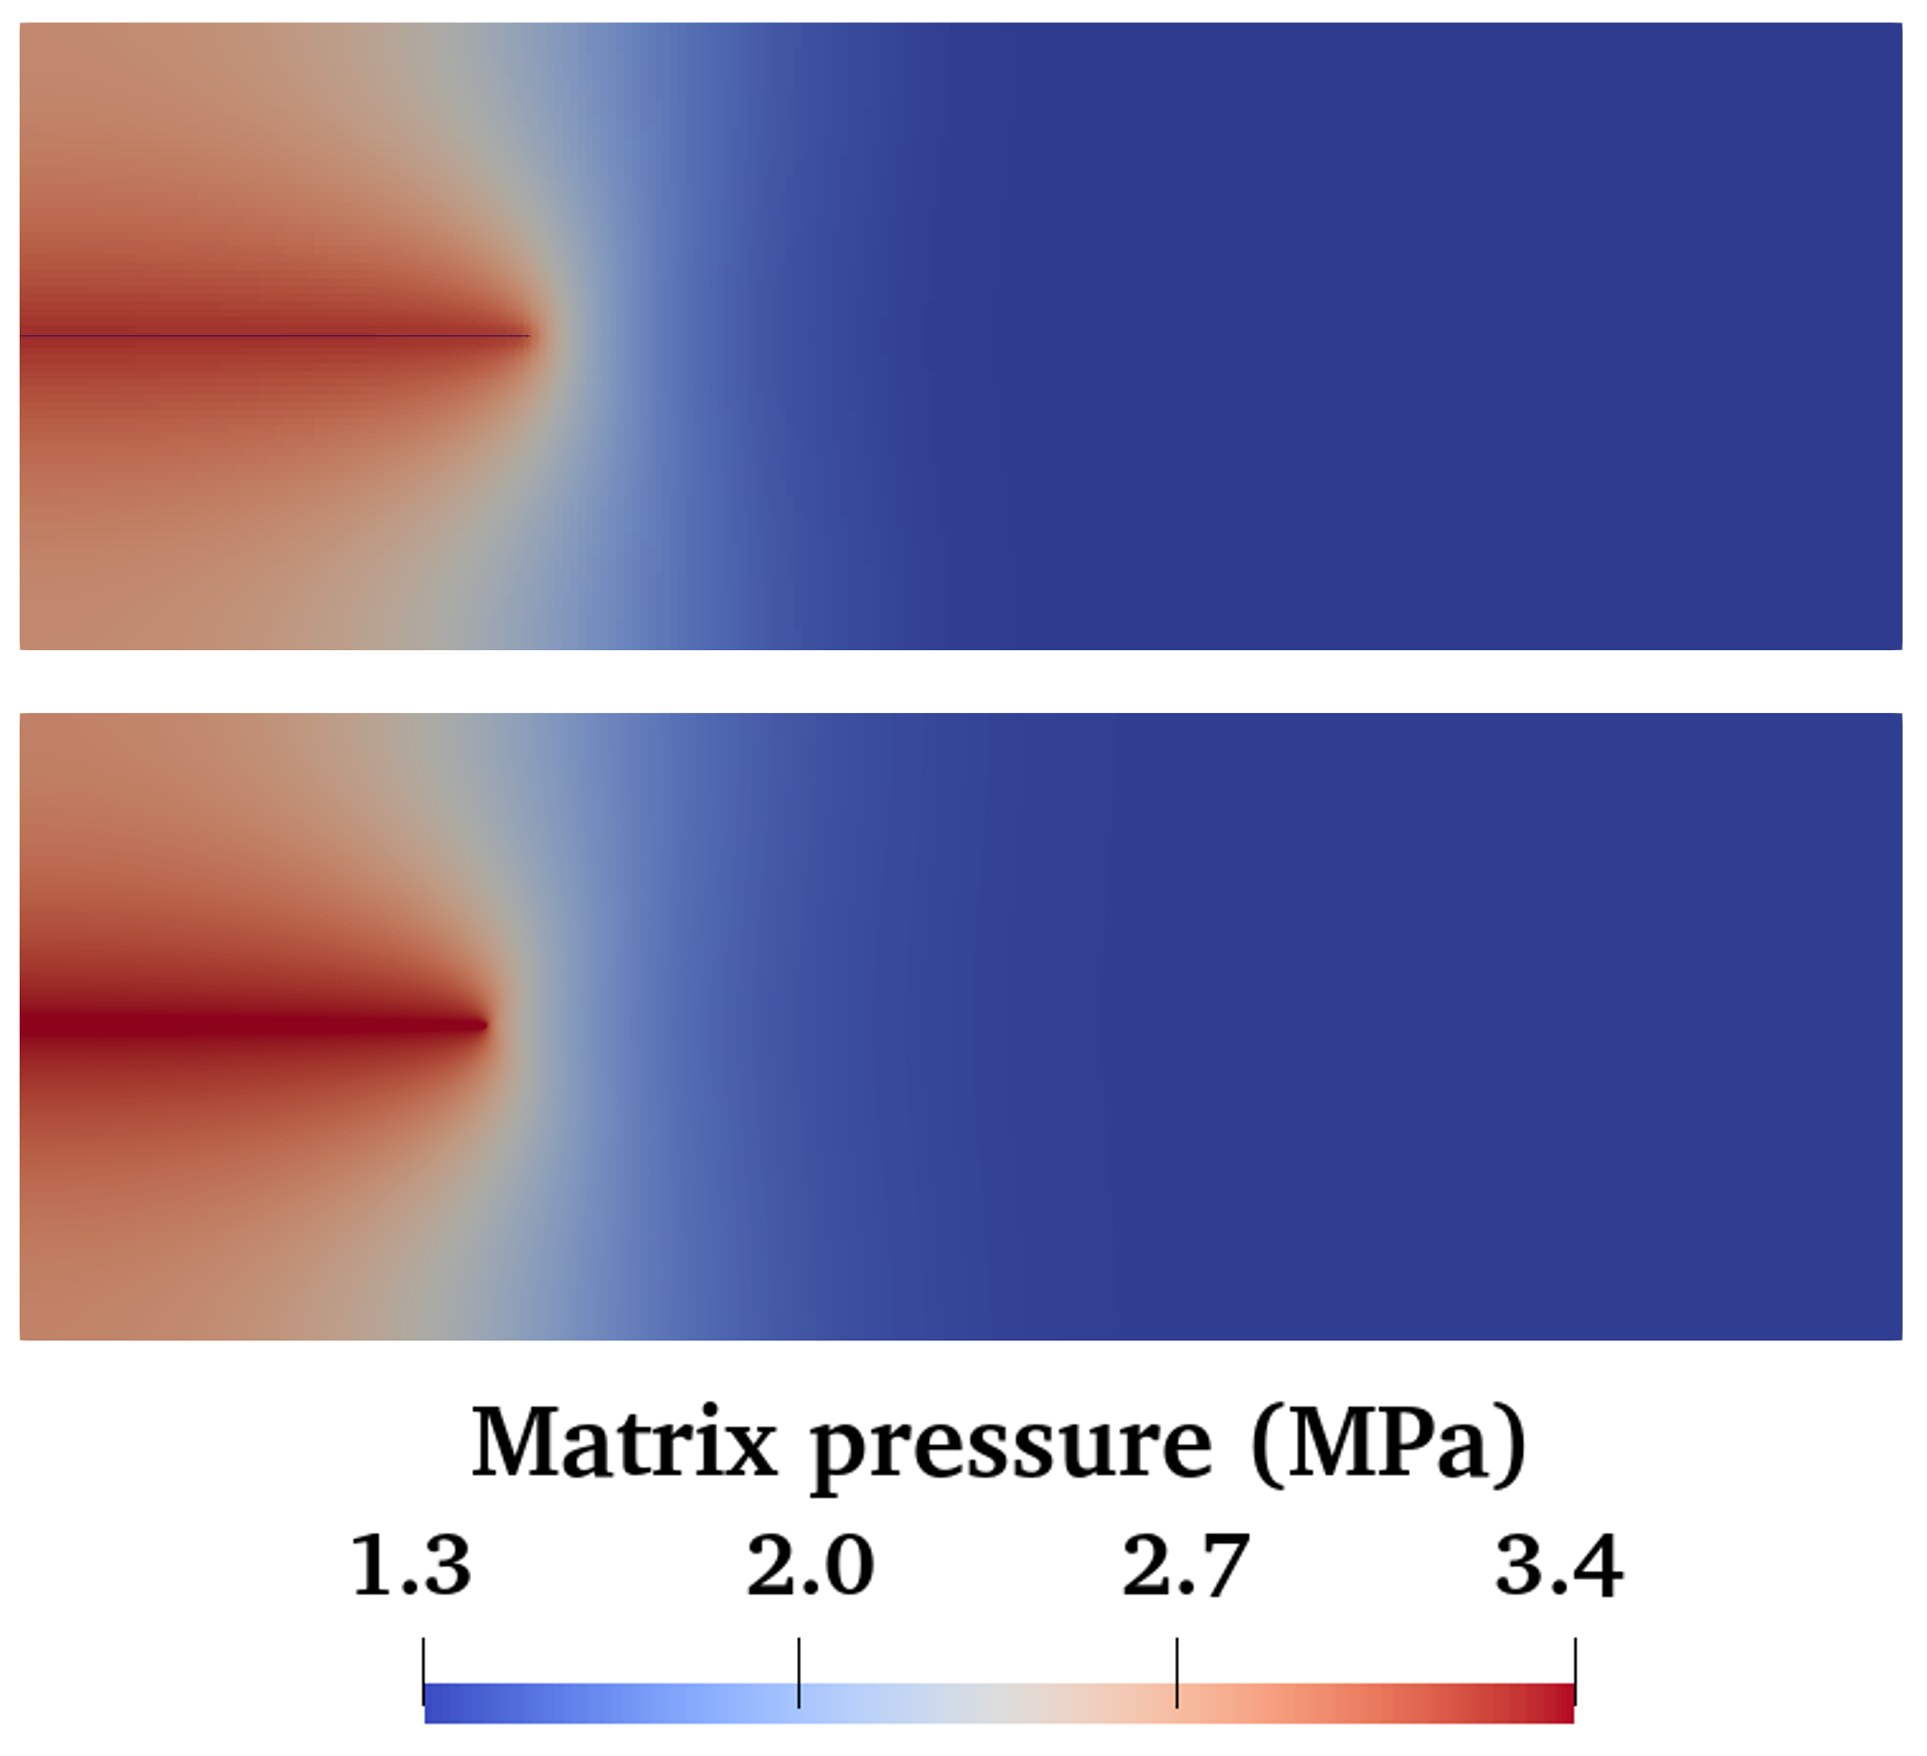
\includegraphics[width=\linewidth]{img/comparison_prob/pressure_fields.png}
  \caption{}
  \label{fig:pressure_snapshot_p2}
\end{subfigure}
  \caption{Fields from the coupled poroelastic-fracture problem, taken at the end of the simulation, contrasting results from the multi-resolution scheme without the driving pressures(top row) to those obtained using a standard phase-field model of fracture in poroelastic media (bottom row).  (a) Contour plots of the damage field.   (b) Contour plots of the pressure field.}
  \label{fig:results_fields_miehe}
\end{figure}

Results for the crack length and inlet pressure as a function of time are provided in Figure~\ref{fig:results_charts_miehe}. Contour plots of the damage and pressure fields for the multi-resolution scheme and the full phase-field formulation are provided in Figure~\ref{fig:results_fields_miehe}.
Despite the numerous differences in the models, the results obtained with the multi-resolution compare very favorably to those obtained using our implementation of the phase-field fracture model \cite{miehe2016phase}.  This is particularly the case when the driving pressures are removed from the multi-resolution method, such that the two phase-field models are as close as possible.    At early times the crack remains stationary, as the pressure at the inlet increases.  At some point the pressure near the crack tip reaches a magnitude that is sufficient to give rise to crack propagation.  After crack propagation begins, the rate of pressure increase begins to decrease with time, as crack growth allows for additional fluid to be accommodated within the fracture. Clearly the phase-field subproblem with a frozen pressure field that acts effectively as a body force is still capable of simulating crack propagation, even when there is flow in the crack and the matrix. It bears emphasis that the multi-resolution scheme does not need to rely on estimations such as \ref{miehe_model_basics},\ref{miehe_model_aperture} to extract an approximation to the aperture from the regularized crack geometry.  

\subsection{Propagation around an inclusion }

\begin{figure}[!htbp]
    \centering
    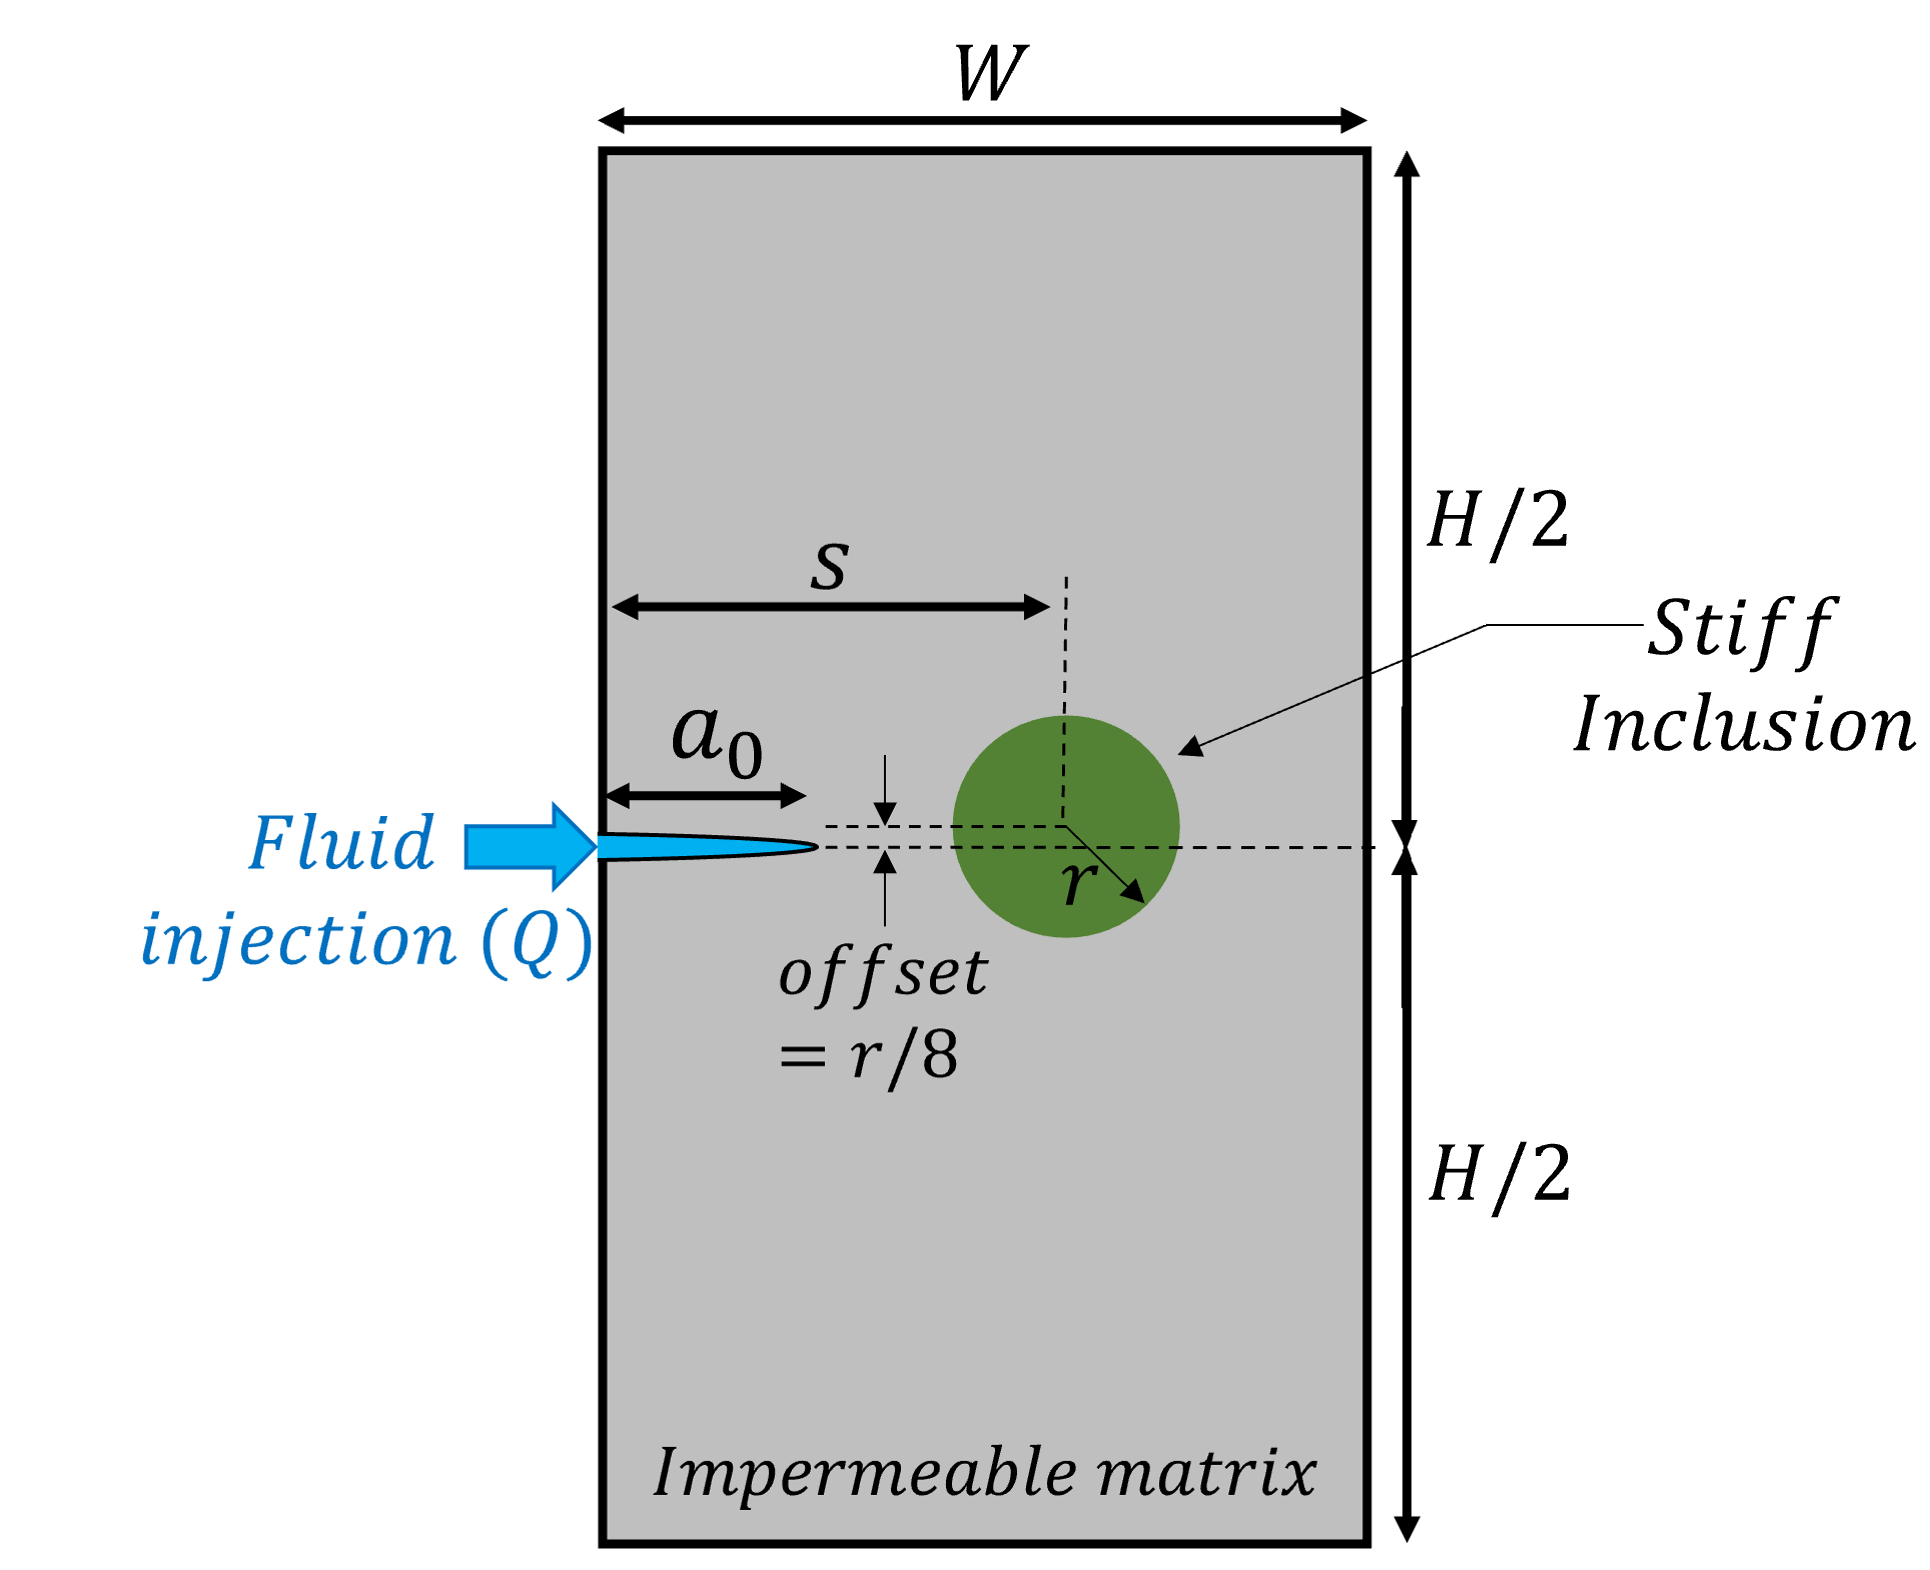
\includegraphics[width=.8\linewidth]{img/inclusion_prob/Inc_prob_updated.png}
    \caption{Geometry for the inclusion problem.}
    \label{fig:description_inc_prob}
\end{figure}

We now consider a problem that gives rise to a non-planar crack evolution.  Specifically, we  investigate the effects of a stiff inclusion on the trajectory of a hydraulically-driven fracture in an impermeable medium. The problem setup is shown in Figure \ref{fig:description_inc_prob}. A circular inclusion of radius $r$ is placed in a rectangular domain, at a distance $s$ from the left boundary, and slightly offset from the axis of symmetry. The inclusion is assumed to have properties that are identical to the matrix, with the exception of the Young's modulus.  
An initial crack of size $a_0$ is placed in the left boundary and a fluid is injected at a constant rate $Q$. The complete set of material properties and geometric parameters are listed in Tables \ref{materials_inclusion} and \ref{geometry_inclusion}.

\begin{table}[ht]
\centering
\caption{Material properties for inclusion problem}
\begin{tabular}[t]{lcc}
\hline
&Value &Unit \\
\hline
Young's modulus ($E$)&9.0&GPa\\
Poisson's ratio ($\nu$)&0.25&--\\
Fluid viscosity ($\mu$)&1.0$\times10^{-12}$&$\text{GPa . s}$\\
Energy release rate ($G_c$)&2.5$\times10^{6}$&$\text{N/m}$\\
\hline
\end{tabular}
\label{materials_inclusion}
\end{table}%

\begin{table}[ht]
\centering
\caption{Problem settings}
\begin{tabular}[t]{lcc}
\hline
&Value &Unit \\
\hline
Phase-Field reg. length ($\ell$)&0.4&m\\
Subdomain size ($L$) &4.0&m\\
Domain width ($W$) &20&$\text{m}$\\
Domain height ($H$) &40&$\text{m}$\\
Initial crack size ($a_0$) &4.0&$\text{m}$\\
Injection rate ($Q$)&1.2$\times10^{-1}$&$\text{m}^2/\text{s}$\\
\hline
\end{tabular}
\label{geometry_inclusion}
\end{table}%

Simulations using the multi-resolution scheme were conducted for three different values of inclusion stiffness, with $h_{local} = \ell/6$ in the local domain, and $h_{global} = 3h_{local}$ in the global domain. The objective was to test how the stiffness of the inclusion influenced the crack trajectory. Consider the following two limiting cases.  When the inclusion is just slightly stiffer than the matrix, one would expect the crack trajectory to remain straight. At the other extreme, when the inclusion is much stiffer, one would expect the crack to propagate around it.  

\begin{figure}[!htbp]
% \centering
\begin{subfigure}{.33\textwidth}
  \centering
  \includegraphics[width=\linewidth]{img/inclusion_prob/2x_bitmap.png}
  \caption{}
  \label{fig:result_2x_inc}
\end{subfigure}%
\begin{subfigure}{.33\textwidth}
  \centering
  \includegraphics[width=\linewidth]{img/inclusion_prob/7x_bitmap.png}
  \caption{}
  \label{fig:result_7x_inc}
\end{subfigure}%
\begin{subfigure}{.33\textwidth}
  \centering
  \includegraphics[width=\linewidth]{img/inclusion_prob/15x_bitmap.png}
  \caption{}
  \label{fig:result_15x_inc}
\end{subfigure}
  \caption{Crack paths for the inclusion problem: (a) 2X stiffer inclusion; (b) 7X stiffer inclusion; and (c) 15X stiffer inclusion. } 
  \label{fig:inclusion_paths}
\end{figure}

The crack paths predicted by the multi-resolution scheme are shown in Figure \ref{fig:inclusion_paths}. The deformed meshes are shown with displacements exaggerated to highlight the crack trajectories. As expected, for an inclusion with much higher stiffness, the crack propagates around it. By contrast, when the stiffness of the inclusion is relatively close to that of the matrix (2X case), the trajectory remains nearly straight. Interestingly, for an intermediate value, where the inclusion is 7 times stiffer than the matrix, the crack trajectory gets deflected, but still goes through the inclusion.  

The pressures at the injection point are plotted as a function of time in Figure \ref{fig:inclusion_pressures}. Due to the very high toughness of the material, they are almost uniform over the crack.  For this problem, we did not observe much sensitivity of the results to the choice of time step size.  By analyzing these curves, we can identify several different stages for this problem.  At early times before any crack propagation begins, we observe a linear increase in pressure with time. Then, as we reach a certain pressure, which we denote as $p_{ref} = 60 \text{ MPa}$, straight crack propagation starts and proceeds until the tip approaches the inclusion. Due to the higher stiffness of the inclusion, the crack arrests and pressure builds up again until it reaches a level that is sufficient to allow propagation to continue.  This is accompanied by a pressure drop that is most pronounced for the higher-stiffness inclusion cases.  

This problem highlights several capabilities of the multi-resoltion scheme, such as the simple handling of crack curving as well as changes in the crack speed, including crack arrest. 
Although we are not aware of any analytical solution for problems like this, the results we have obtained appear to make sense qualitatively. 
\begin{figure}
\centering
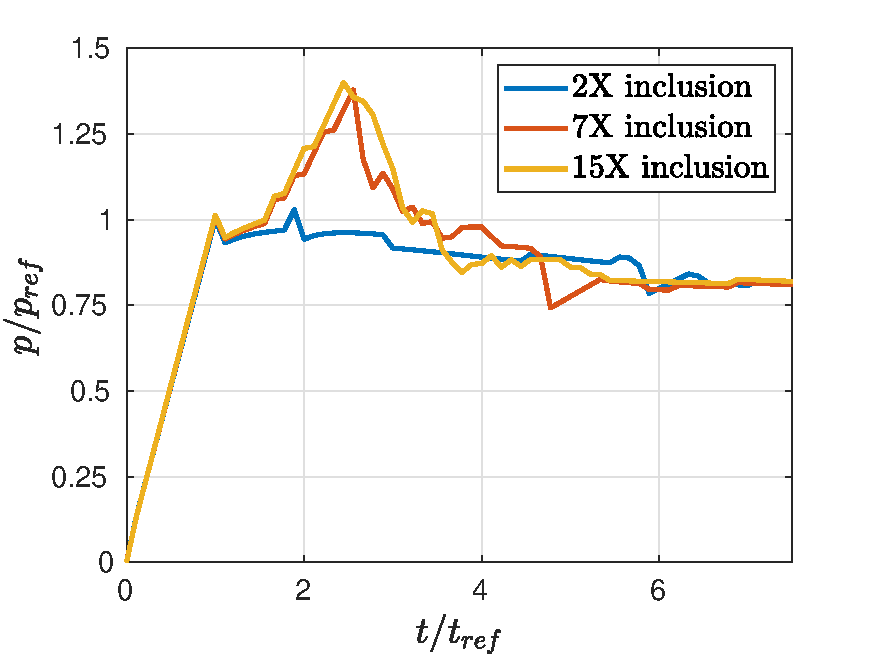
\includegraphics[width=0.5\linewidth]{img/inclusion_prob/inclusion_pressures}
  \caption{Inlet pressure as a function of time for the three inclusion problems, corresponding to inclusions with different stiffnesses. The reference values of the pressure $p_{ref}$ and time $t_{ref}$ were defined as the minimum pressure that led to fracture growth and the associated time, considering the simulated injection rate.} 
  \label{fig:inclusion_pressures}
\end{figure}
\FloatBarrier

